\chapter{El generador del ESP32 como caja negra}
\label{ch:esp32}

% [BORRADOR v2] Primera parte del trabajo y justificación de la segunda.
% Fuentes de las secciones anteriores a sec:esp32_90b: docs/estado_del_arte_trng.md
% (6.1), docs/esp32_linea_base_90b.md (1), docs/plan.md (9),
% firmware/esp32_rng, analysis/esp32_rng, analysis/campana_rng.py,
% results/esp32_rng_agosto, results/esp32_campana_rng y las notas de la
% primera campaña.

Este capítulo es la primera parte del trabajo. Trata el generador hardware
de números aleatorios del ESP32 tal como se lo encuentra un integrador: un
registro que devuelve palabras de 32 bits, detrás del cual el fabricante
nombra dos fuentes de ruido y no cuantifica ninguna. El generador se hace
funcionar en cuatro condiciones de operación en tres campañas de captura;
su salida pasa por una batería SP~800-22 validada con una
autocomprobación, por métricas de Shannon y espectrales y por los
estimadores de SP~800-90B; se construye a su alrededor un recolector de
claves; y una prueba de reinicios abre la caja hasta donde puede abrirse
desde fuera. Toda cifra está medida \meas{} en silicio salvo que se diga
que es calculada. El capítulo termina explicando por qué ninguna de estas
medidas acota la entropía del generador, que es la razón del resto de
este TFM.

\section{El periférico y lo que documenta Espressif}
\label{sec:esp32_periph}

% docs/esp32_linea_base_90b.md 1: ESP32-D0WD-V3, revisión 3.1
El dispositivo es el ESP32 original, un sistema en chip Xtensa LX6 de dos
núcleos; los dos chips medidos aquí son ESP32-D0WD-V3, revisión de silicio
3.1. Según el manual técnico de
referencia~\cite{espressif_trm_esp32}, cada palabra de 32 bits leída de
\texttt{RNG\_DATA\_REG} (dirección 0x3FF75144) es un número verdaderamente
aleatorio, generado a partir del ruido térmico y del desajuste entre
relojes asíncronos; el ruido procede del ADC de alta velocidad de la
radio, del SAR ADC o de ambos, y entra en el generador a través de una
puerta XOR. El SAR ADC aporta 2~bits por ciclo del \texttt{RC\_FAST\_CLK}
de 8~MHz, así que el registro debería leerse a no más de 500~kHz; el ADC
de alta velocidad aporta 2~bits por ciclo del reloj APB de 80~MHz, lo que
permite 5~MHz. Con ninguno de los dos convertidores habilitado, según el
manual, se devuelven números pseudoaleatorios. La guía de
software~\cite{espressif_idf_random} lo expresa en términos operativos: la
salida es verdaderamente aleatoria mientras el Wi-Fi o el Bluetooth están
habilitados, mientras está activa la fuente SAR que enciende
\texttt{bootloader\_random\_enable()} --- que debe apagarse antes de que
la aplicación use el ADC, el I2S o la radio --- o mientras se ejecuta el
bootloader de segunda etapa, y en otro caso ``debe considerarse solo
pseudoaleatoria''. Las aplicaciones leen el generador mediante
\texttt{esp\_random()}, que hace una espera activa entre palabras para que
pueda entrar ruido nuevo, o mediante \texttt{esp\_fill\_random()}, que
llena un búfer con él. En el ESP32 la espera es de 16~ciclos de APB, un
techo de 5~millones de palabras por segundo (\texttt{hw\_random.c}, sin
cambios en este punto desde ESP-IDF 5.2.1 hasta 5.5.2, entre las que
queda la 5.3.2 usada aquí); los 15--75~kHz que cita la guía corresponden a las
esperas más largas programadas para chips posteriores.
% hw_random.c: APB_CYCLE_WAIT_NUM = 16 para el ESP32, 1778 (unos 45 kHz)
% para el ESP32-S3; comprobado en ~/esp/v5.5.2 y en los árboles
% framework-espidf 5.2.1 y 4.4.7 de platformio, y el texto de la guía, el 2026-10-13.

La única validación que publica Espressif es una muestra de 2~GB, leída a
5~MHz con solo el ADC de alta velocidad habilitado, que superó la batería
Dieharder 3.31.1~\cite{espressif_trm_esp32}; los datos no son públicos, y
la muestra cubre solo la condición favorable. No se publica nada sobre el
estado interno con el que se mezcla el ruido, ni ningún modelo del ruido
ni cifra de min-entropía, y la bibliografía consultada solo aplica al
generador SP~800-22 o Dieharder (Sección~\ref{sec:soa_standards}). Para un
integrador es una caja negra con dos entradas documentadas que pueden
encenderse y apagarse, y así es como se mide aquí.

\section{Diseño experimental y captura}
\label{sec:esp32_setup}

% firmware/esp32_rng/main/rng_sampler.c, adc_noise.c, main.c;
% firmware/esp32_rng/sdkconfig.defaults; tiempo de transmisión de unos 25 s
% por condición según docs/esp32_linea_base_90b.md 4
Las dos fuentes documentadas se cruzan como dos factores binarios, lo que
da cuatro condiciones: A, Wi-Fi y ADC; B, solo Wi-Fi; C, solo ADC; D,
ninguna. ``Wi-Fi encendido'' significa la radio arrancada en modo
estación con \texttt{esp\_wifi\_start()}, sin asociarse a ninguna red, ya
que la documentación liga el ruido a que el subsistema de RF esté
habilitado, no al tráfico. ``ADC encendido'' significa una tarea en
segundo plano que mantiene el SAR ADC convirtiendo en el canal~0 del ADC1
(GPIO36, flotante) tan rápido como permite el controlador de conversión
única. Esa no es la fuente SAR documentada, el modo de muestreo de ruido
de \texttt{bootloader\_random\_enable()}, y Espressif no dice si las
conversiones ordinarias llegan al generador; ninguna de las medidas que
siguen puede decidirlo, así que ``ADC encendido'' describe lo que hace el
firmware, no lo que recibe el generador. Las condiciones se ejecutan en el
orden D, C, B, A desde un arranque en frío: D primero, porque una vez que
la radio ha funcionado, un estado con la radio apagada ya no es el de un
dispositivo cuya radio nunca se ha encendido, y cada paso posterior añade
una fuente. El firmware espera 500~ms tras cada cambio, y 200~ms más tras
arrancar la radio, para que cada secuencia pertenezca a una única
condición estacionaria.

Cada condición produce 125\,000 bytes, $10^6$ bits, la longitud mínima que
SP~800-22 recomienda para su batería completa~\cite{bassham_2010_sp80022} y
el número mínimo de muestras de SP~800-90B~\cite{turan_2018_sp80090b}. La
secuencia se genera en RAM con \texttt{esp\_fill\_random()} mientras se
mantiene la condición y solo entonces se transmite, con la tarea del ADC
detenida, porque se comprobó que la actividad del ADC durante ráfagas
serie largas las corrompía; antes de ello, el firmware cronometra la
generación de 64~KiB, y lee la temperatura del chip antes y después. El
flujo es hexadecimal, en tramas que llevan la condición, la repetición,
la temperatura, la tasa y un CRC-32 calculado en el dispositivo; el
anfitrión solo acepta una secuencia si el CRC coincide y la longitud es
exactamente 125\,000 bytes. La consola funciona a 115\,200~baudios, la
única velocidad a la que la salida de la aplicación llegaba de forma
fiable (unos 25~s por condición), con el registro de mensajes en nivel
\texttt{ERROR} porque los mensajes del controlador de Wi-Fi rompían
tramas. Antes del ciclo, \texttt{app\_main} copia un búfer de 4~KiB de la
sección sin inicializar \texttt{.noinit}, el patrón de SRAM de la
Sección~\ref{sec:esp32_harvester}. El firmware está en
\path{firmware/esp32_rng}, y las herramientas, en \path{analysis/esp32_rng}
y \path{analysis/campana_rng.py}.

% capture_log.csv de cada campaña: crc_ok = 1 en las 24 filas
\begin{table}[htbp]
\centering
\caption{Las tres campañas de captura \meas{}. Cada ciclo es un arranque en
frío seguido de las cuatro condiciones en el orden D, C, B, A, de $10^6$
bits cada una.}
\label{tab:esp32_campaigns}
\footnotesize
\begin{tabular}{@{}lllll@{}}
\toprule
Campaña & Fecha & Chip (MAC) & Firmware compilado con & Ciclos \\
\midrule
Primera & 2026-08-04 & ec:e3:34:9a:d1:18 & ESP-IDF 5.3   & 1 \\
Segunda & 2026-09-19 & ec:e3:34:9a:d1:18 & ESP-IDF 5.3.2 & 2 \\
Tercera & 2026-10-12 & a0:dd:6c:0e:fb:4c & ESP-IDF 5.3.2 & 3 \\
\bottomrule
\end{tabular}
\end{table}

Se hicieron tres campañas (Tabla~\ref{tab:esp32_campaigns}). La primera
capturó un ciclo y los patrones de SRAM en el chip de dirección MAC
ec:e3:34:9a:d1:18, que el firmware notifica en el arranque y que se anotó
con los resultados; su registro de captura no tiene columna de MAC.
% resultados de la primera campaña, 2026-08-04: dispositivo ec:e3:34:9a:d1:18
Después, el mismo firmware, recompilado sin cambios, ejecutó dos ciclos
más en ese chip y tres en un segundo chip, a0:dd:6c:0e:fb:4c. Las
veinticuatro secuencias llegaron con la longitud y el CRC correctos. Los
datos están en \path{results/esp32_rng_agosto}, en
\path{results/esp32_campana_rng} y en su subdirectorio
\path{mac_a0dd6c0efb4c}, cada uno con un registro de las temperaturas, las
tasas y los veredictos del CRC. SP~800-22, las métricas de Shannon y el
recolector de las tres secciones siguientes usan la primera campaña; los
estimadores de SP~800-90B de la Sección~\ref{sec:esp32_90b} usan las tres.

\section{La batería SP 800-22}
\label{sec:esp32_sp80022}

% analysis/esp32_rng/nist_sp800_22.py. self_test() repetido el 2026-10-13:
% urandom 15/15, ceros 0/15, alternado 3/15 (pasan frecuencia, frecuencia
% por bloques y sumas acumuladas). El docstring del módulo nombra también
% entradas sesgadas y LFSR de periodo corto, pero self_test() no las ejecuta.
Las quince pruebas de SP~800-22 Rev.~1a~\cite{bassham_2010_sp80022} se
implementaron a partir de las definiciones de la norma en lugar de
tomarse de una biblioteca (\path{analysis/esp32_rng/nist_sp800_22.py}),
tomando los bits del más significativo al menos significativo y
decidiendo cada prueba con $\alpha = 0{,}01$. Las cinco pruebas que
producen varios valores $p$ --- plantillas sin solape, serie, sumas
acumuladas, excursiones aleatorias y su variante --- conservan el mínimo,
de modo que una prueba solo pasa si pasan todas sus partes; la prueba de
plantillas sin solape usa las 8 primeras de las 148 plantillas de
longitud~9 que enumera la norma. Una autocomprobación ejecuta la batería
sobre tres entradas de 125\,000 bytes: los datos de \texttt{os.urandom}
deben pasar con un fallo como máximo, un búfer todo a ceros debe fallar,
y el patrón alternado \texttt{0x55} debe ser rechazado por la prueba de
rachas o por la de entropía aproximada. La supera: los ceros fallan las
quince pruebas, y el patrón alternado falla todas salvo las de
frecuencia, frecuencia por bloques y sumas acumuladas, que una secuencia
perfectamente equilibrada tiene que pasar.

\begin{figure}[htbp]
\centering
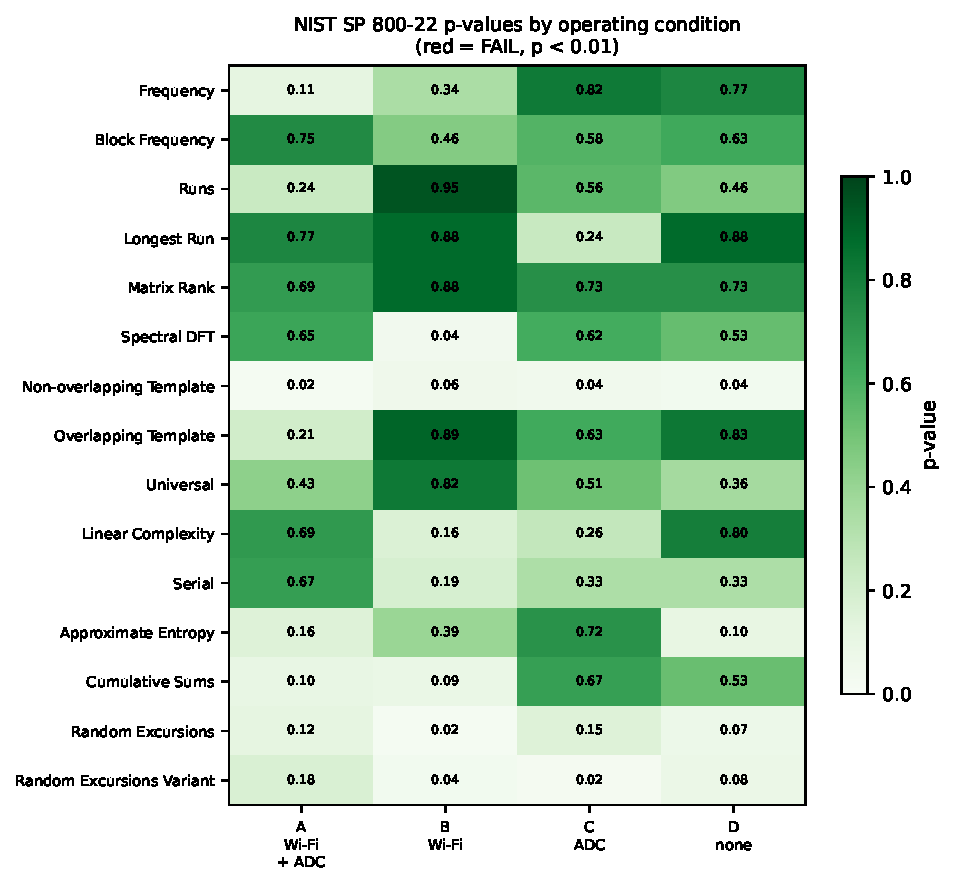
\includegraphics[width=0.8\textwidth]{esp32_nist_heatmap.pdf}
\caption{Valores $p$ de SP~800-22 de las cuatro secuencias de la primera
campaña, uno por condición y prueba, de $10^6$ bits cada una \meas{}. Una
prueba falla por debajo de 0,01; ninguna lo hace. Las pruebas con varios
valores $p$ muestran su mínimo.}
\label{fig:esp32_nist}
\end{figure}

% results/esp32_rng_agosto/nist_summary.csv (15 de 15 en A, B, C, D) y
% nist_results.csv (60 valores p, mínimo 0.0170)
Sobre las cuatro secuencias de la primera campaña la batería pasa las
quince pruebas en las cuatro condiciones (Figura~\ref{fig:esp32_nist}).
La longitud limita lo que eso puede significar. Una fuente perfecta falla
al menos una de quince pruebas con probabilidad
$1-0{,}99^{15} \approx 0{,}14$ (calculado), así que solo un fallo que se
reprodujera indicaría un defecto, y con una secuencia por condición el
análisis de segundo nivel de la norma --- la proporción de secuencias que
pasan y la uniformidad de sus valores $p$ --- no es posible. El menor de
los sesenta valores $p$, 0,017, corresponde a la prueba de plantillas en
la condición~A, y es esperable: el mínimo de $k$ valores $p$ uniformes
tiene una mediana de $1-2^{-1/k}$, que es 0,083 para ocho plantillas y
0,038 para los dieciocho estados de la variante de excursiones
(calculado), y la fila de plantillas (0,017 a 0,055) y la de la variante
(0,020 a 0,176) se sitúan en torno a esas medianas. Nada separa las
condiciones.

Pasar la batería dice que quince estadísticos fijos no distinguen estos
$10^6$ bits de bits independientes y sin sesgo al nivel del 1\,\%. No dice que sean
impredecibles: un generador determinista con una buena función de salida
pasa por diseño, y por eso el NIST decidió en 2022 revisar SP~800-22 y
rechazó su uso para evaluar generadores
criptográficos~\cite{nist_2022_decision}. La condición~D es justo ese caso.
La batería la pasa, Espressif la llama pseudoaleatoria, y la prueba de
reinicios de la Sección~\ref{sec:esp32_90b} muestra que sin el ruido de
arranque es una secuencia fija. La batería sirve aquí como control de
defectos groseros --- sesgo, periodicidad, correlación de corto alcance
--- y no encuentra ninguno.

\section{Entropía de Shannon, tasa y temperatura}
\label{sec:esp32_shannon}

Sobre las mismas cuatro secuencias se calcularon seis métricas más
(\path{analysis/esp32_rng/entropy_analysis.py}). La
Tabla~\ref{tab:esp32_entropy} las da junto al valor que devuelve una
fuente perfecta con la misma longitud, que es la referencia, en lugar del
ideal de una secuencia infinita.

% results/esp32_rng_agosto/entropy_summary.csv; la última fila es calculada
\begin{table}[htbp]
\centering
\caption{Métricas estadísticas de la primera campaña, una secuencia de
$10^6$ bits por condición \meas{}: entropía de Shannon por byte y por bit,
mayor autocorrelación $|r_k|$ para retardos $k$ de 1 a 1000, planitud
espectral de un periodograma de los primeros 65\,536 bits, razón de
compresión de zlib y $\chi^2$ de bytes. La última fila es lo que devuelve
una fuente perfecta con esta longitud (calculado, véase el texto).}
\label{tab:esp32_entropy}
\footnotesize
\begin{tabular}{@{}lllllll@{}}
\toprule
Condición & $H$ (bit/byte) & $H$ (bit/bit) & $\max|r_k|$ & Planitud & zlib & $p$ de $\chi^2$ \\
\midrule
A & 7,99852 & 0,9999982 & 0,00375 & 0,564 & 1,00037 & 0,473 \\
B & 7,99852 & 0,9999993 & 0,00345 & 0,564 & 1,00037 & 0,470 \\
C & 7,99877 & 1,0000000 & 0,00332 & 0,563 & 1,00037 & 0,972 \\
D & 7,99836 & 0,9999999 & 0,00314 & 0,561 & 1,00037 & 0,109 \\
\midrule
Fuente perfecta & $7{,}99853 \pm 0{,}00013$ & $1 - 7\times10^{-7}$ & 0,0034 & 0,561 & $>1$ & uniforme \\
\bottomrule
\end{tabular}
\end{table}

Cada métrica tiene un suelo propio con $10^6$ bits, y la lectura empieza
ahí. La entropía empírica (plug-in) de 125\,000 bytes sobre 256 valores
se queda por debajo de 8~bits incluso para una fuente perfecta, en
$\chi^2_{255}/(2N\ln 2)$, es decir, $0{,}00147 \pm 0{,}00013$~bit; los
cuatro déficits medidos, de 0,0012 a 0,0016~bit, son ese sesgo, y la
entropía de bytes y el $\chi^2$ de bytes son el mismo estadístico en dos
unidades. La entropía por bit reformula la prueba monobit. La
autocorrelación en cada retardo tiene una desviación típica de
$1/\sqrt{n} = 0{,}001$, y el mayor de mil valores así tiene una mediana de
0,0034 para ruido blanco. La planitud de un único periodograma sin
promediar de ruido blanco no es 1 sino $e^{-\gamma} \approx 0{,}561$,
siendo $\gamma$ la constante de Euler, porque cada intervalo de
frecuencia sigue una distribución exponencial. En todas las columnas las
cuatro condiciones quedan donde quedaría una fuente perfecta. Como
SP~800-22, son promedios sobre la salida que una secuencia determinista
puede alcanzar, y la entropía de Shannon no es la magnitud que necesita
una clave: la generación de claves cuenta la min-entropía, el logaritmo
negativo de la probabilidad del resultado más probable, que nunca es
mayor y es el objeto de la Sección~\ref{sec:esp32_90b}.

% throughput_Bps en los tres capture_log.csv: sin la tarea del ADC
% 5214513 a 5218249; con ella 2766632 a 2771781 (primera y segunda
% campañas) y 2703184 a 2705416 (tercera). 64 KiB tardan 12568 us (D)
% y 12559 us (B).
El firmware cronometra la tasa con el temporizador del sistema de
1~$\mu$s sobre 64~KiB, unos 12,6~ms, así que su resolución es mejor que el
0,01\,\% (calculado). En las tres campañas, las doce secuencias sin la
tarea del ADC se generaron a entre 5,21 y 5,22~MB/s ($10^6$~bytes por
segundo), y las doce con ella a 2,77~MB/s en las dos primeras campañas y a
2,70~MB/s en la tercera; la radio cambia la tasa en menos del 0,1\,\%. La
tarea del ADC reduce la tasa a la mitad, por una causa que no se aisló.
Frente al manual, 1,30~millones de palabras por segundo sin la tarea está
por debajo de los 5~MHz del camino de la radio, y de 0,68 a 0,69~millones
con ella está por encima de los 500~kHz del camino SAR: las condiciones A
y C leen de 21,6 a 22,2~Mbit/s mientras que el camino SAR inyecta como
mucho 16~Mbit/s, así que aunque las conversiones de la condición~C
llegaran al generador y cada bit inyectado fuera completamente aleatorio,
detrás de cada bit de salida no podría haber más de 0,72 a 0,74~bit de
ruido nuevo (calculado). El camino de la radio, a 160~Mbit/s, supera casi
cuatro veces la mayor tasa de lectura, 41,7~Mbit/s.

% firmware/esp32_rng/main/temp_monitor.c convierte (F - 32)/1.8 a partir de
% un uint8_t de la ROM; results/esp32_rng_agosto/capture_log.csv solo tiene
% 52.2 y 52.8 (126 y 127 F); temperature_correlation.csv: r = 0.7949,
% p = 0.205; campañas posteriores: los dos capture_log.csv citados arriba.
La temperatura va al final porque su instrumento es el más tosco. El
firmware lee el sensor mediante una función de la ROM no documentada que
devuelve un entero de 8 bits sin calibrar en grados Fahrenheit, así que un
paso es $5/9$~$^\circ$C, 0,556~$^\circ$C. En la primera campaña solo
devolvió 52,2 y 52,8~$^\circ$C, que son 126 y 127~$^\circ$F: todo el rango
de temperatura de la campaña es un paso del sensor. La correlación entre
la entropía de bytes y la temperatura sobre las cuatro secuencias,
$r = 0{,}795$ con $p = 0{,}21$, se calculó por tanto frente al bit menos
significativo del sensor, y no aporta información; no se afirma ningún
efecto de la temperatura, en ningún sentido. Los dos chips identificados
leyeron después de 49,4 a 51,7 y de 61,7 a 64,4~$^\circ$C en la misma
escala sin calibrar, así que chip y temperatura están confundidos. Un
estudio de temperatura necesita un sensor calibrado y un barrido
controlado, y no se hizo ninguno.

\section{Un recolector de claves multifuente}
\label{sec:esp32_harvester}

% firmware/esp32_rng/main/entropy_harvester.c, adc_noise.c, sram_puf.c
Si no se puede confiar en el generador con la radio apagada, un nodo que
mantiene la radio apagada necesita otras fuentes. Esta parte del trabajo
construyó un recolector (\path{firmware/esp32_rng/main/entropy_harvester.c})
que añade dos fuentes del mismo chip cuya disponibilidad complementa la
del generador: el patrón de arranque de la SRAM, presente en cada
encendido antes de que arranque ningún periférico~\cite{holcomb_2009_powerup},
y los bits menos significativos del ADC leyendo una entrada flotante.
Estas pasan por la corrección de Von
Neumann~\cite{vonneumann_1951_various}, que descarta los pares 00 y 11 y
convierte 01 en 0 y 10 en 1, de modo que bits independientes salen sin
sesgo a costa de al menos tres cuartas partes de ellos. Las aportaciones
se acondicionan con SHA-256 en una reserva (\emph{pool}) de 256 bits,
\begin{equation}
\mathrm{pool}_0 = \mathrm{SHA256}\bigl(r \,\|\, \mathrm{SHA256}(S) \,\|\,
a \,\|\, \texttt{"TFM0"}\bigr),
\label{eq:esp32_pool}
\end{equation}
donde $r$ son 32 bytes de \texttt{esp\_fill\_random()}, $S$ el patrón de
SRAM de 4~KiB, $a$ 32 bytes de bits del ADC corregidos y el último campo
una etiqueta que separa este uso del hash de los demás. Cada salida de
32 bytes aplica el hash a la reserva junto con un contador y una lectura
nueva del generador, y después la reserva avanza como un trinquete
(ratchet),
\begin{equation}
o_i = \mathrm{SHA256}(\mathrm{pool} \,\|\, i \,\|\, r_i), \qquad
\mathrm{pool} \leftarrow \mathrm{SHA256}(\mathrm{pool} \,\|\, o_i),
\label{eq:esp32_ratchet}
\end{equation}
de modo que una reserva capturada tras la salida $i$ no permite obtener
las anteriores; un resembrado incorpora a la reserva, mediante el hash,
datos nuevos del generador y del ADC. Concatenar antes de aplicar el hash
da la única garantía que no necesita independencia entre fuentes que
comparten chip, alimentación y temperatura:
$H_\infty(X_1 \| X_2 \| X_3) \geq \max_i H_\infty(X_i)$.

% analysis/esp32_rng/harvester_from_sources.py: entradas puf_boot1.bin y
% condD_rep1.bin, campo del ADC = 32 B del mismo flujo del RNG (sustituto).
% docs/esp32_linea_base_90b.md 1 y 5: el firmware recompilado se detiene en
% la generación de semillas tras el primer ciclo.
% results/esp32_rng_agosto/harvester_validation.csv: 1000 de 1000 únicas,
% chi2 de bytes p = 0.300811, Hamming 128.050 +- 8.027 bits, 7 valores p
% de NIST de 0.147738 a 0.955784.
El recolector se validó fuera de línea. Las semillas producidas en el
dispositivo no se capturaron de forma fiable en la primera campaña, y el
firmware recompilado después se detiene durante la generación de
semillas, un fallo que no se investigó porque las semillas no intervienen
en las demás medidas. La validación reproduce por tanto la construcción
en Python (\path{analysis/esp32_rng/harvester_from_sources.py}) sobre
datos capturados: un patrón de SRAM; la secuencia de la condición~D como
aportación del generador, la peor condición, a propósito; y 32 bytes de
la misma secuencia en lugar del campo del ADC, del que no existe una
captura aparte. De las 1000 semillas de 32 bytes así derivadas, todas son
distintas y sus bytes son uniformes ($\chi^2$ $p = 0{,}30$); la distancia
de Hamming entre dos semillas, sobre 20\,000 pares aleatorios, promedia
128,05 de 256 bits (50,02\,\%) con una desviación típica de 8,03, frente a
128 y 8 para semillas uniformes independientes; y las siete pruebas de
SP~800-22 aplicables a los 256\,000 bits del flujo de semillas pasan, con
$p$ de 0,148 a 0,956.

% calculado a partir de results/esp32_rng_agosto/puf_pc1-4.bin (serie limpia:
% pesos 49.61 a 49.74 %, pares 6.45 a 6.81 %, media 6.63 %, estables
% 28804 de 32768 = 87.90 %) y puf_boot1-5.bin (serie mixta: pesos
% 49.63 a 49.86 %, boot1 frente al resto 49.55 a 49.74 %, pares entre
% boot2-5 6.48 a 7.43 %, estables en boot2-5 28719 de 32768 = 87.64 %,
% la cifra de docs/plan.md 9); 23.9 % en harvester_validation.csv.
La fuente SRAM se caracterizó por separado. Solo un corte de alimentación
vuelve a aleatorizar las celdas, ya que un reinicio que mantiene la
alimentación deja en el búfer lo que escribiera la ejecución anterior, así
que se capturó una serie limpia de cuatro patrones con un ciclo de
alimentación antes de cada uno. Los nueve patrones capturados tienen un
peso de Hamming del 49,6 al 49,9\,\%, y las seis distancias de la serie
limpia van del 6,45 al 6,81\,\%, con una media del 6,63\,\%. La fracción de
celdas estables, las que leen el mismo valor en los cuatro encendidos, se
midió directamente: 87,90\,\% en la serie limpia y 87,64\,\% en los cuatro
encendidos de la primera serie, la mixta, así que unas 4000 de las
32\,768 celdas cambiaron al menos una vez. El primer análisis había
inferido un 93\,\% aproximadamente a partir de la distancia media, que
cuenta con qué frecuencia difieren dos encendidos, no cuántas celdas
difieren alguna vez; la cifra que se usa es la contada
(Sección~\ref{sec:conventions}). La distancia entre arranques del
23,9\,\% calculada inicialmente para la fuente no es una cifra limpia:
promedia diez pares de una serie que mezclaba ciclos de alimentación con
reinicios que mantenían la alimentación, en la que un patrón difiere de
los otros cuatro en el 49,6 al 49,7\,\% de sus bits, como lo harían datos
no relacionados, y los otros seis pares difieren en el 6,5 al 7,4\,\%,
como lo hacen los encendidos de las mismas celdas.

% analysis/esp32_rng/mqtt_tls_demo.py, modo fuera de línea; resultado según
% las notas de la primera campaña (sesión segura).
La validación muestra que la construcción se implementó tal como se
diseñó, no que las semillas lleven entropía. Todas las comprobaciones se
pasan por construcción: el contador hace que cada salida sea distinta
aunque todas las demás entradas fueran constantes, y SHA-256 convierte
entradas distintas cualesquiera en salidas que parecen uniformes y distan
media palabra entre sí. Las entradas de esta validación lo ilustran. El
campo de SRAM fue un mismo patrón para las 1000 semillas --- el primero
de la serie mixta, que no es un estado de encendido --- y la única
entrada que cambiaba entre semillas era la salida de la condición~D, que
la prueba de reinicios muestra que es una secuencia fija una vez
eliminado el ruido de arranque. La entropía de una semilla es como mucho
$\min(256, H_\infty)$ bits, siendo $H_\infty$ la min-entropía de las
entradas, y esta no se midió para ninguna de ellas. Un peso del 50\,\% no
cambia esto: el 88\,\% de las celdas de la SRAM son una huella fija,
conocida por cualquiera que haya leído el patrón una vez, y acotar lo que
aporta el 12\,\% restante requeriría muchos más encendidos y un modelo de
las celdas. El recolector es una arquitectura cuya salida es al menos tan
fuerte como su mejor fuente, no una fuente de entropía medida. Una
demostración fuera de línea de su uso previsto
(\path{analysis/esp32_rng/mqtt_tls_demo.py}) expande una semilla en una
clave de sesión con HKDF-SHA256~\cite{krawczyk_2010_hkdf} y protege un
mensaje con AES-256-GCM, rechazando un mensaje reenviado y otro
manipulado; ejercita la criptografía, y la clave hereda la entropía de la
semilla sin añadir ninguna.

\section{La referencia del ESP32 frente a SP 800-90B}
\label{sec:esp32_90b}

O8 pide una comparación numérica con el ESP32, y la mitad puede cerrarse
sin la placa: el lado de la referencia. Las
Secciones~\ref{sec:esp32_sp80022} y~\ref{sec:esp32_shannon} aplicaron
SP~800-22 y la entropía de Shannon a la primera campaña; los estimadores
de SP 800-90B se aplican aquí a las tres, que en conjunto dan seis
repeticiones de $10^6$ bits por condición, tres en cada uno de los dos
chips del mismo modelo (ESP32-D0WD-V3). Otras dos capturas con la radio
apagada, de $3{,}52\times10^6$ y $8{,}38\times10^6$ bits, se tomaron con
el firmware verificador del Capítulo~\ref{ch:ch5_verification}. Las
veintiséis se pasaron por la implementación de referencia del \ac{NIST} de
los estimadores de SP 800-90B~\cite{nist_ea_github, turan_2018_sp80090b}
(versión 1.1.8), por la vía IID y por la vía no IID, en el formato
binario que la norma prescribe para fuentes de bits. La
Tabla~\ref{tab:esp32_90b} recoge el resultado.

\begin{table}[htbp]
\centering
\caption{El generador del ESP32 frente a los estimadores de SP 800-90B \meas{}.
Condiciones A--D: seis repeticiones de $10^6$ bits cada una, tres en cada
uno de los dos chips, media y rango sobre las repeticiones; E y F:
capturas únicas de $3{,}5\times10^6$ y $8{,}4\times10^6$ bits. El techo es
el valor más alto que el estimador del valor más común (MCV) puede
devolver para una fuente perfectamente uniforme de esa longitud con un
99\,\% de confianza; la cifra no IID es el mínimo de los diez estimadores
de la Sección~6.3 de la norma, y la última columna nombra el estimador que
la fijó (veces de seis). Los veredictos de la vía IID se discuten en el
texto.}
\label{tab:esp32_90b}
\footnotesize
\begin{tabular}{@{}llrrll@{}}
\toprule
Captura & Condición & $H$ (IID) & Techo & $H$ (no IID) & Limitante \\
\midrule
A & Wi-Fi + ADC & 0,9954 & 0,9963 & 0,844 (0,812--0,877) & Compresión 5, Lag 1 \\
B & Wi-Fi       & 0,9951 & 0,9963 & 0,862 (0,824--0,898) & Compresión 5, LRS 1 \\
C & ADC         & 0,9952 & 0,9963 & 0,836 (0,812--0,867) & Compresión 6 \\
D & ninguna     & 0,9957 & 0,9963 & 0,857 (0,832--0,916) & Compresión 5, Colisión 1 \\
E (verificador) & ninguna & 0,9977 & 0,9980 & 0,867 & Compresión \\
F (verificador) & ninguna & 0,9982 & 0,9987 & 0,911 & Compresión \\
\bottomrule
\end{tabular}
\end{table}

La resolución va primero, como en todo este trabajo. El estimador MCV
devuelve $-\log_2 p_u$ con $p_u = \hat p + 2{,}576\sqrt{\hat p(1-\hat p)/N}$,
de modo que ni siquiera una fuente perfecta puede puntuar por encima de
0,9963 con $10^6$ bits, de 0,9980 con $3{,}5\times10^6$ ni de 0,9987 con
$8{,}4\times10^6$. Cada una de las veintiséis capturas queda a menos de
0,0035 de ese techo, y ninguna implica un sesgo de unos superior a
$2{,}4\sigma$, que es lo que se observa en veintiséis extracciones de una
fuente sin sesgo.

La vía IID necesita una calibración antes de que puedan leerse sus
veredictos. De las cincuenta y dos ejecuciones (veintiséis capturas en los
formatos de bits y de bytes), cuatro fallan una sola prueba, nunca el
mismo fichero en ambos formatos: una prueba de permutación en cada formato
y dos pruebas $\chi^2$ en el formato de bytes. La frecuencia con que datos
buenos fallan estas pruebas a esa misma longitud no es el $10^{-3}$
nominal, así que se midió, ejecutando la misma herramienta sobre 1000
ficheros de 125\,000 bytes y 200 ficheros de $10^6$ bits del generador del
sistema operativo. En el formato de bytes, la batería de permutación falla
en el 1,9\,\% de los ficheros buenos y el par $\chi^2$ en el 2,4\,\%; en el
formato de bits, la batería de permutación falla en el 2,5\,\% y el par
$\chi^2$ en ninguno de los 200. La cifra de $\chi^2$ se rastreó hasta su
causa reimplementando ambas pruebas, lo que reproduce los cincuenta y dos
valores $p$ de la herramienta hasta la sexta cifra decimal, y ejecutándolas
sobre 5000 ficheros buenos. La prueba de independencia del formato de
bytes reparte 62\,500 pares sin solape entre 65\,536 celdas y agrupa celdas
hasta que cada grupo espera cinco cuentas, pero a esta longitud su $p$ no
es uniforme: la mediana es 0,175 en lugar de 0,5, y cae por debajo de
$10^{-3}$ en el 1,7\,\% de los ficheros, diecisiete veces la tasa nominal.
Las otras tres pruebas $\chi^2$ están bien calibradas, y el defecto
desaparece a partir de $10^6$ bytes. Frente a estas tasas, los fallos del
ESP32 no tienen nada de particular: un fallo de permutación en veintiséis
ejecuciones en formato de bytes donde se esperan 0,49 ($P = 0{,}39$), dos
fallos $\chi^2$ donde se esperan 0,62 ($P = 0{,}13$), y un fallo de
permutación en el formato de bits donde se esperan 0,65 ($P = 0{,}48$). En
un chip, la prueba de independencia de bytes dio $p < 0{,}05$ en seis
capturas de doce, frente a 2,9 esperadas; agrupar las capturas de cada
chip, donde la prueba está calibrada y es más potente, da valores $p$
empíricos de 0,82 y 0,96 en ese chip para pares de bytes alineados con la
palabra de 32 bits y desplazados un byte, y de 0,38 y 0,86 en el otro, así
que no hay dependencia entre bytes vecinos. El suceso más raro es el fallo
de bondad de ajuste de la primera captura de la condición~D
($p = 2{,}4\times10^{-4}$): esa prueba falla en el 0,04\,\% de los ficheros
buenos, así que un fallo así en veintiséis tiene una probabilidad cercana
al 1\,\%. No se reprodujo en las cinco capturas posteriores de la misma
condición ($p = 0{,}32$ a $0{,}96$) ni en E y F, y se registra como azar;
la advertencia de Espressif de que la aleatoriedad del generador no está
garantizada sin la radio o el ADC sigue en pie como una advertencia que
estas pruebas no ven. Formalmente, un único fallo retira la hipótesis IID
para esa captura; como la cifra que se retiene es la no IID, nada de lo
que sigue depende de ello. Leída con su calibración, la vía IID encuentra
la salida del ESP32 indistinguible de una fuente binaria de entropía
completa con este tamaño de muestra. Es el mismo veredicto que dio
SP 800-22, alcanzado por otro camino, y dice lo mismo: no se ve nada mal.

La vía no IID dice otra cosa, y leerla bien importa más que el número. En
veinticinco de las veintiséis capturas, su mínimo lo fija uno de tres
estimadores --- compresión, colisión o subcadena repetida más larga --- con
0,81 a 0,92 bit por bit; en la restante, el predictor Lag, con 0,88; los
estimadores MCV y de Markov nunca bajan de 0,99. Se sabe que esos tres
estimadores son conservadores con datos casi uniformes~\cite{zhu_2017_analysis};
los predictores de Kelsey, McKay y S\"onmez Turan~\cite{kelsey_2015_predictive}
se introdujeron precisamente porque los estimadores anteriores de la norma
juzgan mal fuentes de ese tipo. Las repeticiones muestran que esto es un
comportamiento de los estimadores y no una propiedad de las condiciones.
La estimación por compresión tiene una desviación típica de 0,02 a 0,04
\emph{dentro} de una condición, tan grande como el 0,03 que separa las
medias de las cuatro condiciones, y un análisis de la varianza de un factor
sobre cada uno de los once estimadores no encuentra diferencia entre
condiciones: el $p$ más pequeño es 0,083, para el predictor MultiMCW, por
encima del 0,05 sin corregir y muy por encima del 0,0045 que exigen once
pruebas. Lo mismo vale entre chips. Agrupando las condiciones, que no
difieren, ningún estimador separa las doce capturas de cada chip al nivel
corregido; el $p$ más pequeño, 0,047 para MCV, corresponde a una
diferencia de 0,0007 bit por bit junto al techo de resolución, y un valor
por debajo de 0,05 entre once pruebas es lo que da el azar. El mínimo no
IID es 0,852 en un chip y 0,847 en el otro: con dos dispositivos, la
referencia no depende de cuál se mida, a la resolución de estos
estimadores. La captura más grande añade una segunda muestra del efecto
de la resolución: en el formato de bytes, su estimador limitante es la
prueba de $t$-tupla con $t = 2$, que devuelve 7,39 bits por byte porque
$10^6$ bytes contienen demasiado pocos de los 65\,536 pares posibles para
que el más frecuente sea representativo, exactamente como le ocurre al
techo del MCV con $t = 1$. Ningún estimador resuelve con seis
repeticiones diferencia alguna entre Wi-Fi encendido, ADC encendido y
ninguno de los dos, y no se afirma ninguna.

La prueba de reinicios de la Sección~3.1.4 de la norma responde a lo que
la estadística anterior no puede: si un generador no tiene ruido propio,
su salida tras un reinicio en frío debe repetirse. Un firmware dedicado
leyó 1024~bytes con \texttt{esp\_fill\_random} como primera acción de la
aplicación, con la radio y el ADC apagados (condición~D), y el chip de MAC
a0:dd:6c:0e:fb:4c se reinició 1000 veces por su patilla de habilitación;
la ROM de arranque notificó un reinicio por encendido todas las veces. Dos
variantes comparten la aplicación y difieren solo en el bootloader de
segunda etapa: el de serie, que inyecta ruido del SAR ADC en el generador
durante unos 126~ms mientras se ejecuta, y el mismo bootloader con esa
llamada desviada a una función vacía en tiempo de enlazado, lo que
confirma el desensamblado. Otras tres variantes hacen una segunda lectura
tras arrancar el Wi-Fi como en las condiciones A y B, sin asociarse a
ninguna red, y esperar 200~ms, con cada uno de los dos bootloaders; la
tercera es un control que espera el mismo tiempo sin tocar la radio, de
modo que la lectura cae en el mismo tick del planificador. La
Tabla~\ref{tab:esp32_restart} recoge el resultado.

\begin{table}[htbp]
\centering
\caption{Prueba de reinicios del generador del ESP32 \meas{}: 1000 reinicios
en frío por variante, un chip. $H_r$ y $H_c$ son el mínimo de los
estimadores no IID sobre el conjunto de filas y el conjunto de columnas de
la norma (1000 reinicios $\times$ 1000 bits); la prueba falla cuando
cualquiera de los dos queda por debajo de la mitad de la estimación
inicial $H_I$, la cifra no IID más baja de este chip en la misma condición
(0,838 bit por bit en D, 0,859 en B). El formato de bytes da los mismos
veredictos. Los solapes son reinicios cuya salida aparece desplazada
dentro de la de otro, todos idénticos palabra por palabra. Las lecturas
tardías caen entre 352 y 412~ms después de que arranque la aplicación, la
mayoría a 352~ms.}
\label{tab:esp32_restart}
\footnotesize
\begin{tabular}{@{}llrrrl@{}}
\toprule
Bootloader & Lectura & $H_r$ / $H_c$ & Distintas & Solapes & Veredicto \\
\midrule
De serie & en el arranque, radio apagada & 0,898 / 0,854 & 1000 & 0 & pasa \\
Sin ruido de arranque & en el arranque, radio apagada & 0,024 / 0,813 & 759 & 5424 & falla \\
Sin ruido de arranque & tardía, radio apagada (control) & 0,024 / 0,808 & 760 & 5632 & falla \\
Sin ruido de arranque & tardía, Wi-Fi encendido & 0,831 / 0,845 & 1000 & 0 & pasa \\
De serie & tardía, Wi-Fi encendido & 0,844 / 0,807 & 1000 & 0 & pasa \\
\bottomrule
\end{tabular}
\end{table}

Con el bootloader de serie el generador pasa en ambos formatos, y las
1000 salidas difieren entre sí exactamente como lo harían datos
aleatorios: la distancia de Hamming media entre dos reinicios es de 4096,0
bits de 8192, frente a $4096 \pm 45$ esperados. Sin el ruido de arranque
falla de forma tajante, y los datos muestran por qué. Cada reinicio es una
ventana sobre una única secuencia fija, leída desde un punto de partida
ligeramente distinto: dondequiera que el comienzo de la salida de un
reinicio aparece dentro de la de otro, desplazado unas pocas palabras de
32 bits, todo el solape coincide palabra por palabra, 5424 veces sin una
sola diferencia. Lo único que cambia entre reinicios es el instante en que
la aplicación empieza a leer, que varía en unos pocos miles de ciclos de
reloj de un arranque al siguiente. Eso vale entre 6,5 bits por reinicio,
la cota de la norma a partir de la salida más repetida, y 10,8 bits si
todos los puntos de partida fueran igual de probables, de 8192 bits leídos.
Con la radio y el ADC apagados el generador no tiene ruido propio, y la
afirmación de Espressif de que entonces su salida es solo
pseudoaleatoria~\cite{espressif_idf_random} queda confirmada directamente,
cosa que ninguna prueba estadística sobre un flujo continuo podría hacer.
De ello se siguen dos consecuencias. Las capturas de la condición~D de la
Tabla~\ref{tab:esp32_90b} son la salida de un generador determinista
sembrado durante el arranque: los estimadores les acreditan 0,85 bit por
bit, tanto como con la radio encendida, mientras que su entropía física es
como mucho la que inyectó el bootloader, que esos estimadores no miden. Y
una aplicación que deriva una clave justo después del arranque con la
radio apagada depende por completo del ruido del bootloader de serie; sin
él, la clave podría adivinarse en unos pocos miles de intentos, el
problema del arranque en frío descrito por Blanco-Romero
et al.~\cite{blancoromero_2026_entropy}.

Las filas con radio responden a la otra mitad de la afirmación de
Espressif. Sin el ruido de arranque, arrancar el Wi-Fi basta para que la
prueba pase: las 1000 salidas son todas distintas, no se comparte ninguna
ventana, y los 289 pares de reinicios que leían valores idénticos antes de
arrancar la radio leen 289 valores diferentes después. La temporización
por sí sola no lo explica. El control espera el mismo tiempo y lee en el
mismo tick del planificador, con un instante de lectura que varía otro
tanto (3824 frente a 5260 ciclos de reloj entre los reinicios que
comparten el tick), y se repite exactamente como en el arranque: 760
salidas distintas, 5632 solapes idénticos, unos 1700 estados. Con tan
pocos estados, los 797 reinicios que comparten un tick en la variante con
radio mostrarían unas 180 repeticiones solo por temporización; no muestran
ninguna. Sin la radio, el generador no recibe ruido en sus primeros
350~ms de funcionamiento; con la radio, sí. Lo que la prueba no da es
cuánta entropía por bit aporta la radio: los 0,83 bit por bit validados
son la cifra de los estimadores, con su sesgo habitual, no una medida del
ruido de la radio. No se ha encontrado en la bibliografía consultada una
prueba de reinicios del generador del ESP32.

\section{Lo que una caja negra puede decir y lo que no}
\label{sec:esp32_lessons}

Todos los instrumentos estadísticos aplicados al generador del ESP32 dan
la misma respuesta. SP~800-22 pasa las quince pruebas en las cuatro
condiciones; las métricas de Shannon, de autocorrelación, espectrales y de
compresión quedan donde quedaría una fuente perfecta con esta longitud;
la vía IID de SP~800-90B, leída con su calibración, encuentra la salida
indistinguible de una fuente binaria de entropía completa; y la vía no
IID acredita de 0,81 a 0,92~bit por bit, sin ninguna diferencia entre
condiciones o entre chips que resuelva algún estimador. Ninguna de estas
cifras distingue la condición~D, en la que Espressif dice que el
generador es pseudoaleatorio, de la condición~A, en la que están activas
las dos fuentes documentadas.

La prueba de reinicios es la única medida que lo hace, porque plantea una
pregunta física y no estadística: ¿se repite la salida cuando el
generador vuelve a arrancar desde el mismo estado? Sin el ruido de
arranque y con la radio apagada se repite, palabra por palabra; con la
radio encendida, no. El generador no tiene ruido propio con la radio y el
ADC apagados, y la radio sí le inyecta ruido. Las cifras de SP~800-90B de
la condición~D son, por tanto, el veredicto de los estimadores sobre la
continuación determinista de una semilla de arranque: una cifra
estadística, que no puede acreditarse como entropía física. Lo mismo
vale, de forma menos visible, para las demás condiciones. La prueba de
reinicios muestra que la radio inyecta ruido, no cuánto; para las
condiciones A y C ni siquiera está establecido que las conversiones del
ADC lleguen al generador, y según las propias tasas del manual el camino
SAR no podría aportar un bit de ruido nuevo por bit de salida a la tasa a
la que se leyó el generador.

Lo que falta no es una prueba mejor sino un tipo distinto de
conocimiento: un modelo de la fuente --- qué proceso físico produce la
aleatoriedad, y con qué parámetros --- y una medida de esos parámetros que
acote la min-entropía por debajo. Ninguna de las dos cosas puede
obtenerse desde fuera del ESP32: sus fuentes de ruido, su estado interno
y su posprocesado no están documentados, y los estimadores de
SP~800-90B se diseñaron para muestras de ruido en bruto, no para la
salida de un bloque que puede estar ya acondicionado. Por eso la segunda
parte de este trabajo construye el generador en lugar de medir el de
otro. El Capítulo~\ref{ch:ch3_entropy} parte de la física de un oscilador
en anillo, extrae su jitter y lo convierte, mediante un modelo validado,
en una cota inferior de la min-entropía; los capítulos siguientes
construyen y verifican el motor en torno a esa fuente. El ESP32 sigue en
el trabajo con otros dos papeles: su cifra no IID es la referencia de la
comparación de la Sección~\ref{sec:esp32_ref}, y su biblioteca
criptográfica es la implementación independiente con la que se verifica
el motor.
